\documentclass[11pt]{amsart}
\usepackage{tikz}


\begin{document}
\title{TikZ Practice}
\author{Wooyoung Chin}
\maketitle

\begin{enumerate}
\item
A right isosceles triangle.
\begin{center}
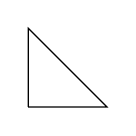
\begin{tikzpicture}
\draw (0,0) -- (1,0) -- (0,1) -- (0,0);
\end{tikzpicture}
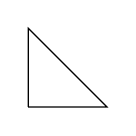
\begin{tikzpicture}
\draw (0:0) -- (0:1) -- (90:1) -- (0:0);
\end{tikzpicture}
\end{center}

\item
Arrows, thickness, and more.
\begin{center}
\begin{tikzpicture}
\draw [->, thick, dashed, red] (0,0) -- (0,2);
\draw [->, ultra thick, dotted, cyan] (0,0) -- (2,0);
\end{tikzpicture}
\end{center}

\item
Curves.
\begin{center}
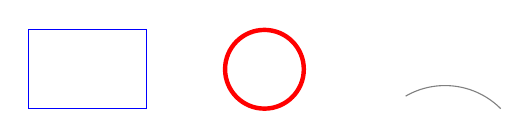
\begin{tikzpicture}
\draw [blue] (0,0) rectangle (1.5,1);
\draw [red, ultra thick] (3,0.5) circle [radius=0.5];
\draw [gray] (6,0) arc [radius=1, start angle=45, end angle=120];
\end{tikzpicture}
\end{center}

\item
Including texts.
\begin{center}
\begin{tikzpicture}
\draw (90:1.5) node {Wei};
\draw (210:1.5) node {Shu};
\draw (-30:1.5) node {Wu};
\draw (0:0) -- (30:1.5);
\draw (0:0) -- (150:1.5);
\draw (0:0) -- (-90:1.5);
\end{tikzpicture}
\begin{tikzpicture}
\draw[<->] (-2,0) node [left] {$-\infty$}
-- (0,0) node [below] {$\mathbf{R}$}
-- (2,0) node [right]
{$+\infty$};
\end{tikzpicture}

\end{center}

\item
Plotting functions.
\begin{center}
\begin{tikzpicture}
	\draw [->] (-1.5*pi,0) -- (1.5*pi,0) node [below right] {$x$};
	\draw [->] (0,-1.5) -- (0,1.5) node [left] {$y$};
	\draw [domain=-1.5*pi:1.5*pi] plot (\x, {sin(\x r)});
\end{tikzpicture}
\end{center}

\item
Filling up areas.
\begin{center}
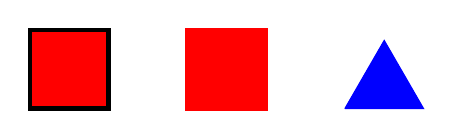
\begin{tikzpicture}
\draw [fill=red,ultra thick] (0,0) rectangle (1,1);
\draw [fill=red,ultra thick,red] (2,0) rectangle (3,1);
\draw [blue, fill=blue] (4,0) -- (5,0) -- (4.5,{sqrt(3)/2})--(4,0);
\end{tikzpicture}
\end{center}

\item
Overlaying areas.
\newcommand{\drawbox}[1]{%
\draw[shift=#1, fill=yellow] (0:0) -- (30:.5) -- (90:.5) -- (150:.5) -- (0:0);
\draw[shift=#1, fill=red] (0:0) -- (150:.5) -- (210:.5) -- (270:.5) -- (0:0);
\draw[shift=#1, fill=blue] (0:0) -- (270:.5) -- (330:.5) -- (30:.5) -- (0:0);
}
\begin{center}
\begin{tikzpicture}
\drawbox{(90:0.5)}
\drawbox{(30:0.5)}
\drawbox{(0:0)}
\drawbox{(-30:0.5)}
\end{tikzpicture}
\end{center}

\item
Regular polygons.
\newcommand{\regpoly}[1]{%
\begin{tikzpicture}
	\draw (-90:1)
	\foreach \n in {1,...,#1} {
		-- (-90+\n*360/#1:1)
	};
\end{tikzpicture}
}

\begin{center}
\regpoly{4}
\regpoly{5}
\regpoly{6}
\regpoly{7}
\regpoly{8}
\end{center}

\end{enumerate}


\end{document}